\section{Análise descritiva do tratamento}
\label{sec:resultados_descritica}

Esta seção apresenta uma análise descritiva sistemática dos dados utilizados para investigar os efeitos do lobbying na atividade parlamentar dos deputados do Parlamento Europeu. A abordagem adotada segue uma estratégia analítica multinível, iniciando com padrões agregados gerais e progredindo para análises desagregadas mais específicas. Esta progressão metodológica permite compreender tanto as tendências globais quanto os mecanismos específicos que operam no nível individual e temporal.

O conjunto de dados constitui um painel balanceado que combina informações sobre atividade parlamentar (perguntas) e intensidade de lobbying (reuniões) para 1.727 deputados ao longo de 63 meses, de agosto de 2019 a outubro de 2024 em 9 domínios de política pública. Esta estrutura temporal permite capturar variações tanto na dimensão \textit{cross-sectional} (entre deputados e domínios) quanto longitudinal (evolução temporal), fornecendo a base empírica necessária para estratégias de identificação causal robustas. A tabela \ref{tab:mep_treatment_stats} apresenta as estatísticas agregadas do painel de dados.

\begin{table}[htbp]
    \centering
    \caption{Estatísticas agregadas de tratamento por deputado}
    \label{tab:mep_treatment_stats}
    \begin{tabular}{lr}
    \toprule
    \textbf{Estatística} & \textbf{Valor} \\
    \midrule
    Total de reuniões & 235.638 \\
    Total de perguntas & 118.238 \\
    Total de deputados únicos & 1{,}727 \\
    Deputados que receberam tratamento & 804 \\
    Taxa de tratamento por deputado (\%) & 46{,}5\% \\
    \midrule
    \textbf{Entre deputados tratados:} & \\
    Reuniões médias por deputado & 293{,}1 \\
    Reuniões medianas por deputado & 109{,}0 \\
    Desvio padrão & 468{,}9 \\
    \midrule
    \textbf{Correlação agregada:} & \\
    Correlação reuniões-perguntas & 0{,}05 \\
    \bottomrule
    \end{tabular}
\end{table}

Considerando a unidade de análise a tríade MEP-domínio-mês, temos 979.209 observações com taxa de completude de 100\%. Esta estrutura balanceada é metodologicamente vantajosa, pois elimina preocupações com viés de seleção decorrente de atrito amostral e garante que as estimativas não sejam distorcidas por padrões de observações ausentes.

A cobertura temporal de agosto de 2019 a outubro de 2024 é particularmente relevante por abranger períodos de intensa atividade legislativa europeia, incluindo a transição entre legislaturas e eventos político-econômicos significativos. Destaca-se, nesse intervalo, o impacto da pandemia de COVID-19, que afetou profundamente tanto a dinâmica da atividade parlamentar quanto as estratégias de lobbying. A pandemia resultou em mudanças substanciais nos modos de trabalho do Parlamento Europeu, com a adoção de sessões remotas e restrições a reuniões presenciais, o que pode ter alterado padrões de interação entre deputados e grupos de interesse. Assim, a análise cobre não apenas períodos de normalidade institucional, mas também um contexto de crise sanitária global, permitindo investigar como choques exógenos desse tipo influenciam o comportamento político e o lobbying.

A \autoref{fig:time_series} apresenta a evolução temporal das variáveis principais no nível mais agregado, revelando padrões que são fundamentais para compreender a dinâmica do sistema político europeu ao longo do período estudado.

\begin{figure}[htbp]
\centering
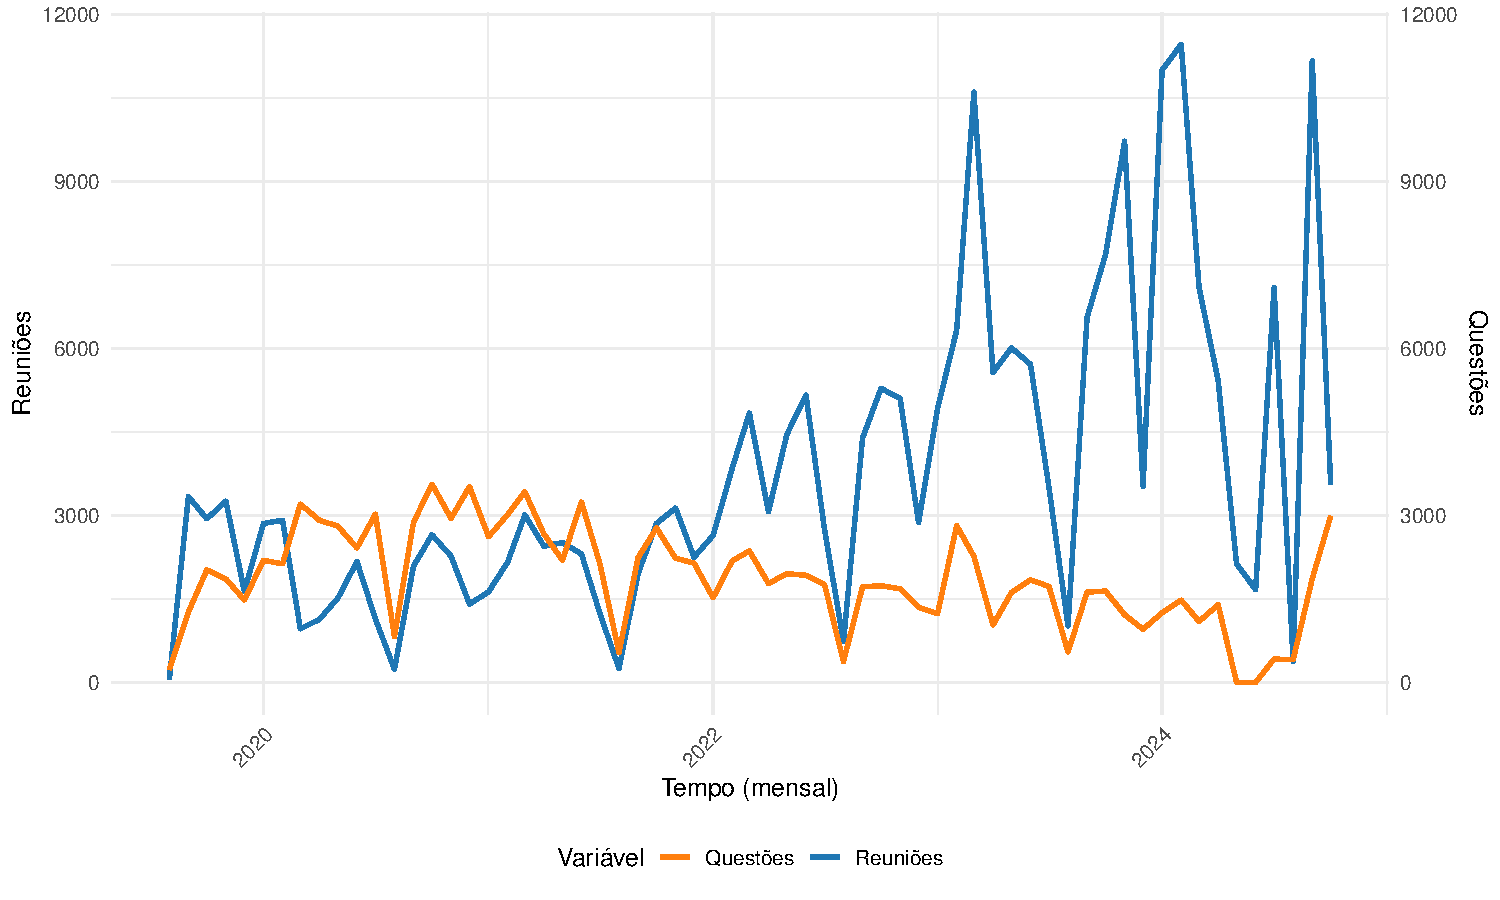
\includegraphics[width=\textwidth]{figures/descriptive_plots/fig1_time_series_meetings_questions.pdf}
\caption{Evolução temporal da atividade parlamentar e de lobbying}
\label{fig:time_series}
% \note{O painel superior esquerdo mostra os totais mensais agregados de perguntas e reuniões. O painel superior direito apresenta as médias mensais por observação MEP-domínio. O painel inferior esquerdo mostra a evolução da proporção de observações com atividade de lobbying. O painel inferior direito apresenta a estabilidade da correlação contemporânea entre as variáveis ao longo do tempo.}
\end{figure}

A análise da evolução temporal (Figura \ref{fig:time_series}) revela uma dinâmica complexa na interação entre a atividade de lobbying (reuniões) e a atividade parlamentar (perguntas). O padrão mais saliente é a \textbf{divergência de tendências} a partir do início de 2022. Enquanto o volume de perguntas parlamentares (linha laranja) permanece relativamente estável ao longo de todo o período, oscilando dentro de uma faixa consistente - com leve tendência de queda -, o número de reuniões de lobby (linha azul) apresenta um crescimento acentuado e um aumento expressivo da volatilidade a partir de 2022.

A estabilidade no número de perguntas parlamentares sugere que este instrumento funciona mais como uma ferramenta de rotina da fiscalização e posicionamento político, menos elástica às flutuações de curto prazo da agenda legislativa mais contenciosa. Além disso, ambas as séries exibem uma clara \textbf{sazonalidade}, com quedas de atividade que correspondem aos períodos de recesso do calendário parlamentar, um fator institucional que molda o ritmo do trabalho político.

Do ponto de vista metodológico, estes padrões são cruciais. A tendência de crescimento no lobby e a sazonalidade em ambas as séries justificam a inclusão de efeitos fixos de tempo (ex: mês-ano) nos modelos econométricos, para controlar choques temporais comuns e variações sazonais que poderiam confundir a estimação dos efeitos. A divergência entre as séries a partir de 2022 também sugere a importância de se testar a estabilidade dos parâmetros do modelo ao longo do tempo.


% \subsection{Padrões de participação: análise agregada por deputado}

Complementando a análise temporal, é fundamental examinar os padrões de participação no nível individual dos deputados. Esta perspectiva agregada revela a distribuição da atividade de lobbying entre os parlamentares e fornece insights sobre a concentração e heterogeneidade dos fenômenos estudados.



As \autoref{fig:proportion_meetings}, \autoref{fig:correlation_meetings_questions} e \autoref{fig:meetings_hist} apresentam uma análise dos padrões de participação agregados por deputado, revelando aspectos da distribuição da atividade de lobbying no Parlamento Europeu que impactam a identificação causal.


\begin{figure}[htbp]
    \centering
    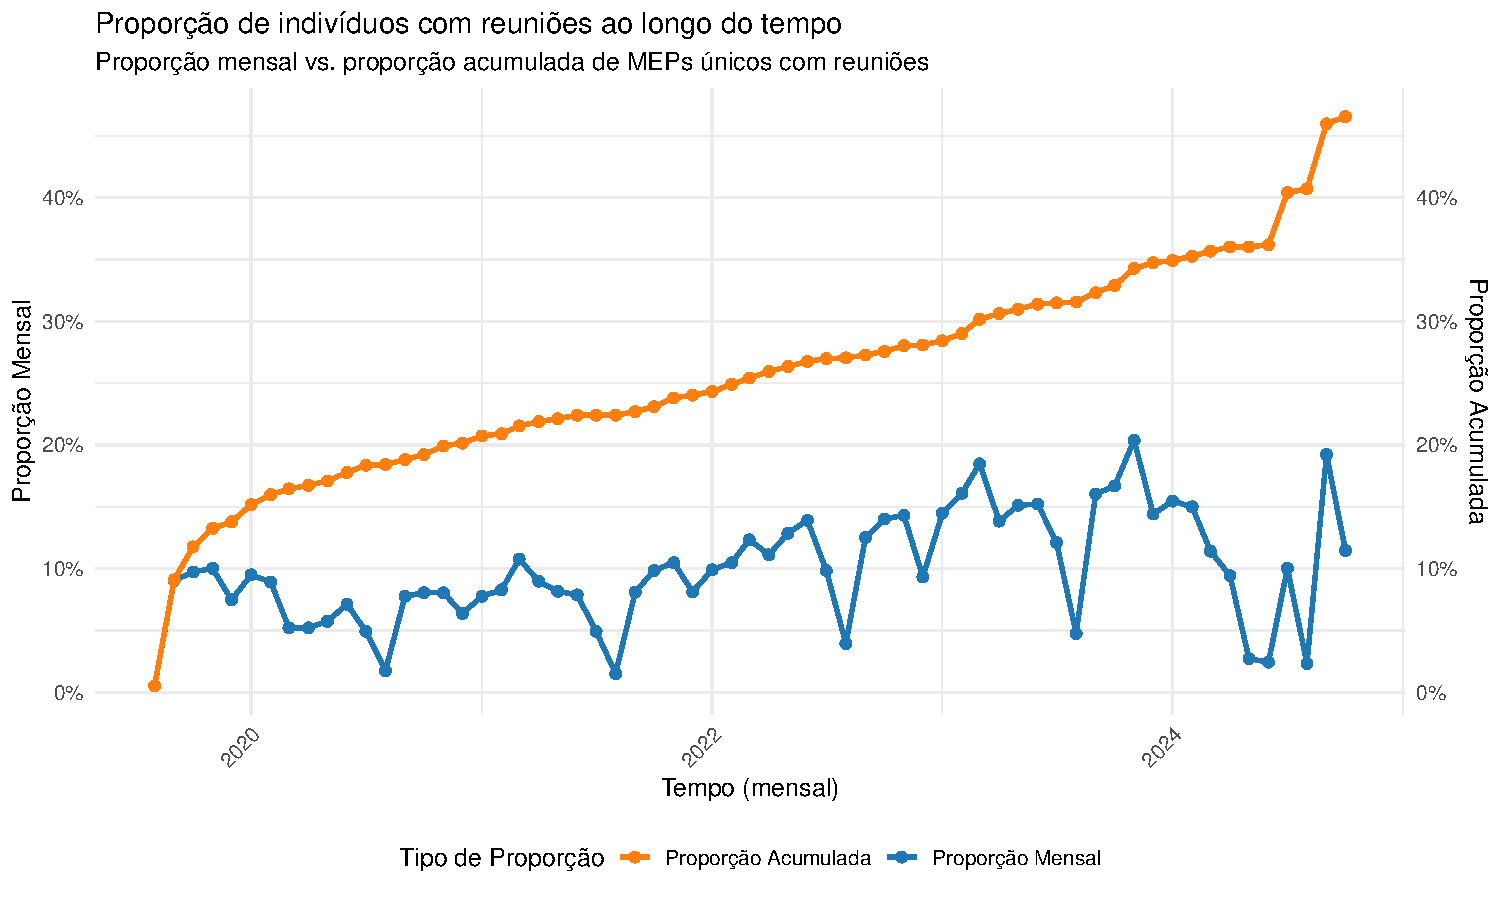
\includegraphics[width=\textwidth]{figures/descriptive_plots/fig2_proportion_meetings.pdf}
    \caption{Evolução temporal da proporção de \acrshort{mpe}s que participaram de reuniões de lobbying}
    \label{fig:proportion_meetings}
    % \note{O painel superior esquerdo mostra os totais mensais agregados de perguntas e reuniões. O painel superior direito apresenta as médias mensais por observação MEP-domínio. O painel inferior esquerdo mostra a evolução da proporção de observações com atividade de lobbying. O painel inferior direito apresenta a estabilidade da correlação contemporânea entre as variáveis ao longo do tempo.}
\end{figure}

\begin{figure}[htbp]
    \centering
    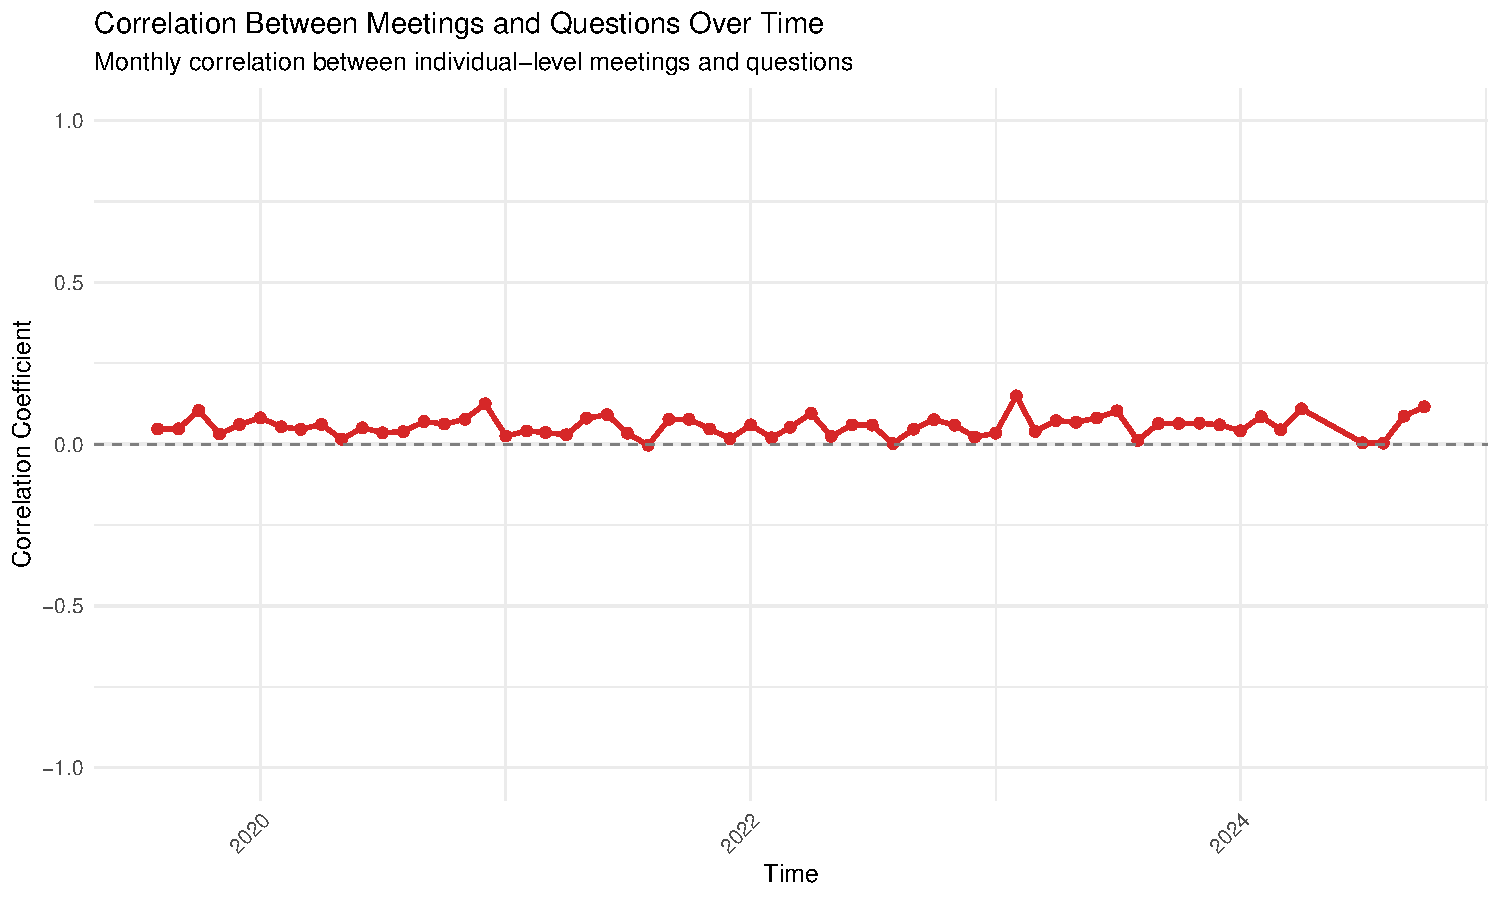
\includegraphics[width=\textwidth]{figures/descriptive_plots/fig3_correlation_meetings_questions.pdf}
    \caption{Evolução temporal da correlação entre reuniões e perguntas}
    \label{fig:correlation_meetings_questions}
    % \note{O painel superior esquerdo mostra os totais mensais agregados de perguntas e reuniões. O painel superior direito apresenta as médias mensais por observação MEP-domínio. O painel inferior esquerdo mostra a evolução da proporção de observações com atividade de lobbying. O painel inferior direito apresenta a estabilidade da correlação contemporânea entre as variáveis ao longo do tempo.}
\end{figure}

\begin{figure}[htbp]
    \centering
    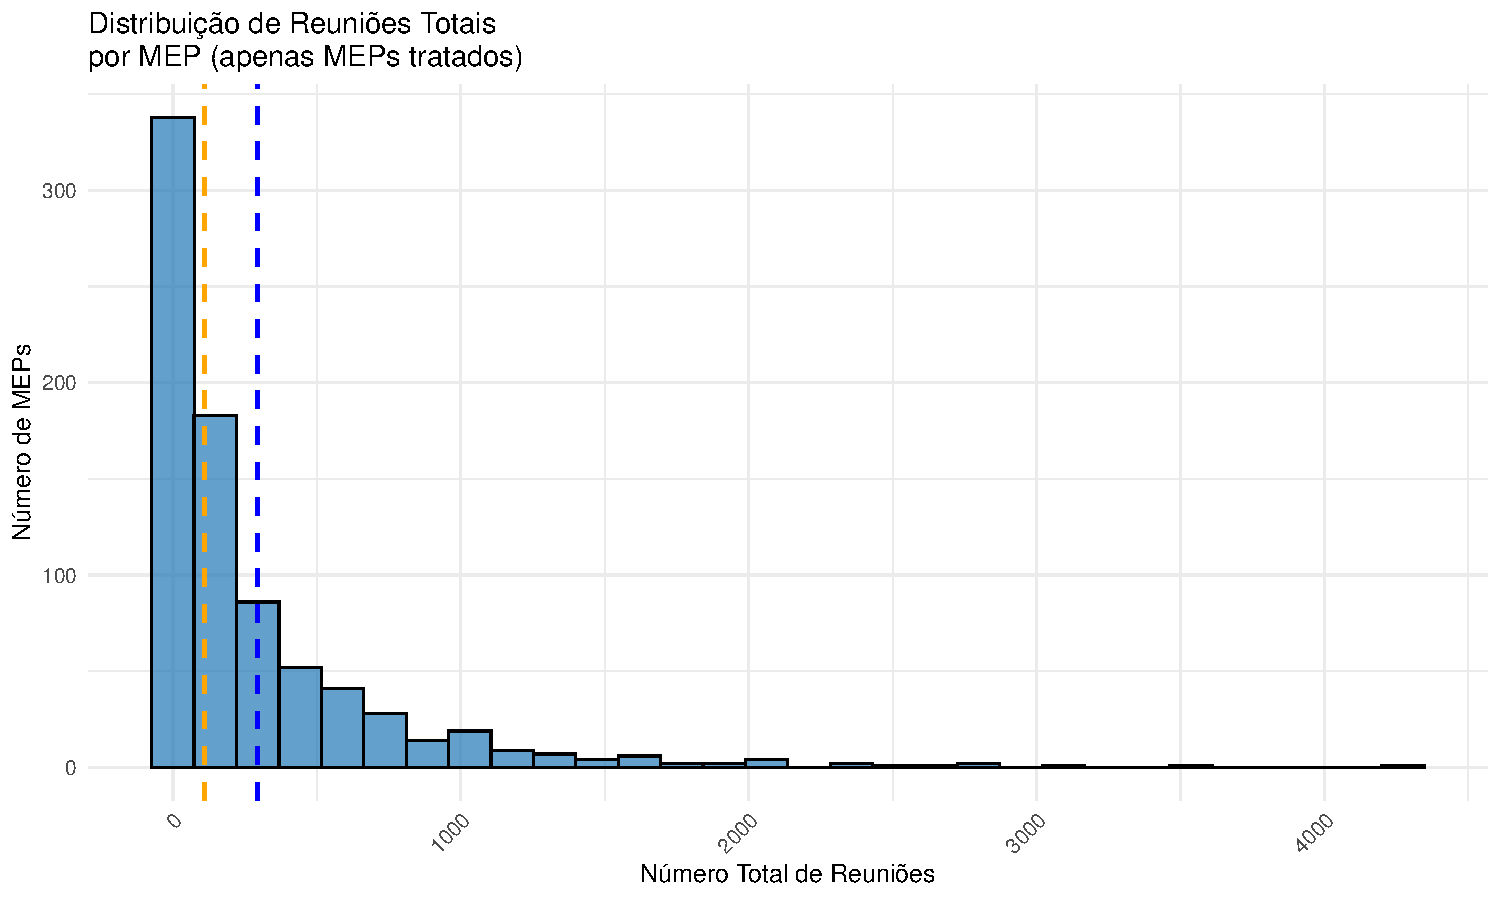
\includegraphics[width=\textwidth]{figures/descriptive_plots/fig3.1_meetings_hist.pdf}
    \caption{Distribuição de reuniões por \acrshort{mpe}}
    \label{fig:meetings_hist}
    % \note{O painel superior esquerdo mostra os totais mensais agregados de perguntas e reuniões. O painel superior direito apresenta as médias mensais por observação MEP-domínio. O painel inferior esquerdo mostra a evolução da proporção de observações com atividade de lobbying. O painel inferior direito apresenta a estabilidade da correlação contemporânea entre as variáveis ao longo do tempo.}
\end{figure}


A análise revela três características fundamentais da distribuição de tratamento. Primeiro, existe \textbf{participação substancial mas não universal}: 46,5\% dos deputados (804 de 1.727) receberam pelo menos uma reunião de lobbying durante o período estudado. Esta proporção indica que o lobbying é um fenômeno disseminado mas não ubíquo no sistema parlamentar europeu.

Segundo, observa-se \textbf{concentração extrema} na intensidade de tratamento. Entre os deputados que receberam lobbying, a distribuição é altamente assimétrica: enquanto a mediana é de 109 reuniões por deputado, a média é de 293,1 reuniões, indicando que uma minoria de parlamentares concentra uma quantidade desproporcional da atividade lobista. O caso extremo de um deputado com 4.274 reuniões ilustra esta concentração.

Terceiro, a \textbf{correlação agregada} entre reuniões e perguntas totais por deputado é surpreendentemente baixa (0,05), contrastando com correlações mais elevadas observadas no nível temporal. Este padrão sugere que os efeitos do lobbying podem ser mais evidentes em frequências temporais específicas do que em padrões de atividade agregados de longo prazo.


Estes padrões agregados têm implicações importantes para a identificação causal. A concentração do tratamento em uma minoria de deputados sugere que estratégias de identificação baseadas em variação \textit{cross-sectional} podem sofrer de poder estatístico limitado. Simultaneamente, a variação substancial na intensidade de tratamento entre deputados tratados fornece fonte valiosa de identificação para estimativas de dose-resposta.

A baixa correlação agregada, combinada com correlações temporais mais elevadas, indica que a identificação causal pode beneficiar-se de estratégias que explorem variação temporal \textit{within-individual} ao invés de \textit{cross-sectional between-individual}. Esta evidência preliminar orienta a especificação de modelos com efeitos fixos de deputado para controlar heterogeneidade não observada invariante no tempo.


\subsection{Heterogeneidade entre domínios de política pública}

A terceira dimensão da análise agregada examina a variação entre domínios de política pública. Esta heterogeneidade setorial é teoricamente relevante porque diferentes áreas de política podem apresentar características distintas em termos de complexidade técnica, interesse econômico e organização de grupos de pressão, afetando tanto a demanda por lobbying quanto a responsividade parlamentar.

% \paragraph{Padrões de tratamento por domínio}

A análise da Tabela \ref{tab:domain_treatment_rates} revela uma heterogeneidade sistemática entre os domínios de política pública, que se manifesta de forma distinta na penetração e na intensidade do lobby.

\begin{table}[htbp]
    \centering
    \caption{Taxa de tratamento por domínio: deputados únicos que receberam lobbying}
    \label{tab:domain_treatment_rates}
    \begin{tabularx}{\textwidth}{>{\raggedright\arraybackslash}X c c c c c c}
        
        \hline
        \tiny{\textbf{Domínio}} & \tiny{\textbf{MEPs}} & \tiny{\textbf{MEPs}} & \tiny{\textbf{Reuniões}} & \tiny{\textbf{Perguntas}} & \tiny{\textbf{Penetração}} & \tiny{\textbf{Intensidade}} \\
        & \tiny{\textbf{(A)}} & \tiny{\textbf{Tratados (B)}} & \tiny{\textbf{(C)}} & \tiny{\textbf{}} & \tiny{\textbf{(B/A \%)}} & \tiny{\textbf{Média (C/B)}} \\
        \hline 
        \tiny{Tecnologia} & \tiny{1727} & \tiny{789} & \tiny{32.067} & \tiny{9.918} & \tiny{45,69} & \tiny{40,64} \\
        \tiny{Economia e Comércio} & \tiny{1727} & \tiny{788} & \tiny{34.762} & \tiny{13.884} & \tiny{45,63} & \tiny{44,11} \\
        \tiny{Assuntos Externos e Segurança} & \tiny{1727} & \tiny{783} & \tiny{28.041} & \tiny{13.462} & \tiny{45,34} & \tiny{35,81} \\
        \tiny{Infraestrutura e Indústria} & \tiny{1727} & \tiny{782} & \tiny{32.795} & \tiny{10.544} & \tiny{45,28} & \tiny{41,94} \\
        \tiny{Meio Ambiente e Clima} & \tiny{1727} & \tiny{777} & \tiny{32.038} & \tiny{14.665} & \tiny{44,99} & \tiny{41,23} \\
        \tiny{Saúde} & \tiny{1727} & \tiny{769} & \tiny{23.868} & \tiny{20.602} & \tiny{44,53} & \tiny{31,04} \\
        \tiny{Educação} & \tiny{1727} & \tiny{738} & \tiny{18.670} & \tiny{2.949} & \tiny{42,73} & \tiny{25,30} \\
        \tiny{Direitos Humanos} & \tiny{1727} & \tiny{727} & \tiny{17.194} & \tiny{26.482} & \tiny{42,10} & \tiny{23,65} \\
        \tiny{Agricultura} & \tiny{1727} & \tiny{711} & \tiny{16.203} & \tiny{5.732} & \tiny{41,17} & \tiny{22,79} \\
        \hline
        
    \end{tabularx}
\end{table}



Em termos de \textbf{penetração} (a proporção de deputados que recebem ao menos uma reunião), a variação entre os domínios é moderada, oscilando entre 41,2\% (Agricultura) e 45,7\% (Tecnologia). Essa pequena amplitude sugere que o lobby, como prática, é uma atividade transversal e disseminada por todo o Parlamento Europeu, não se restringindo a nichos específicos. Ainda assim, o padrão é teoricamente consistente: domínios ligados à regulação econômica e de alta complexidade (Tecnologia, Economia e Comércio, Infraestrutura) apresentam as maiores taxas, refletindo os elevados interesses em jogo \cite{mahoney_lobbying_2007}.

A heterogeneidade torna-se muito mais acentuada quando se analisa a \textbf{intensidade média do tratamento} (o número médio de reuniões por deputado "tratado"). Aqui, a variação é extrema: um deputado ativo em "Economia e Comércio" recebe, em média, 44 reuniões, quase o dobro das 23 reuniões de um deputado ativo em "Agricultura". Esta é a dimensão onde a alocação estratégica de recursos se torna mais evidente. Domínios com altas consequências econômicas e complexidade técnica atraem não apenas um pouco mais de lobistas, mas um esforço de influência massivamente mais concentrado, validando a tese de que os recursos de lobby fluem para as arenas de maior saliência e complexidade regulatória \cite{kluver_informational_2012}.

É notável também o contraste entre a intensidade do lobby e o volume de atividade parlamentar. O domínio de "Direitos Humanos", por exemplo, apresenta o maior número de perguntas parlamentares (26.482), mas uma das menores taxas de penetração e a segunda menor intensidade de lobby. Este padrão sugere que a dinâmica política varia conforme o tema. Enquanto domínios econômicos são caracterizados por um lobby intenso e técnico, temas de grande apelo público como "Direitos Humanos" podem ser mais influenciados por estratégias de \textit{advocacy} e pela sinalização política dos parlamentares através de instrumentos como as perguntas, em vez do lobby direto medido por reuniões.

% Inflação de zeros
A unidade de análise adotada — deputado-domínio-mês — revela uma alta proporção de observações com valor zero (>92\%) tanto para reuniões quanto para perguntas. Contudo, esta "inflação de zeros" não representa um problema estatístico, mas sim uma característica substantiva do comportamento parlamentar: a \textbf{especialização temática}. Como documentado na literatura \cite{schiller1995senators, burden2015personal}, parlamentares concentram sua atividade em um subconjunto de domínios, resultando em zero atividade na maioria das combinações deputado-domínio. A atividade de lobby, por sua vez, segue essa especialização, direcionando-se aos parlamentares já ativos em cada tema.

A natureza "artificial" dessa inflação de zeros é confirmada quando os dados são agregados. Ao considerar apenas os domínios em que um deputado demonstra alguma atividade, a proporção de zeros cai para 47,1\% para perguntas e 55,8\% para reuniões. Em um nível agregado por domínio-mês, a inflação de zeros torna-se negligível (3,2\% e 0\%, respectivamente), indicando que há atividade constante em todos os domínios quando se considera o conjunto de parlamentares relevantes. Portanto, a escolha do modelo econométrico \acrshort{ppml} justifica-se pela natureza da variável dependente (dados de contagem com excesso de zeros), evitando os vieses de modelos lineares com transformações logarítmicas.

A análise descritiva delineia um ecossistema de lobbying no \acrshort{pe} caracterizado por \textit{(i)} dinamismo temporal acentuado, \textit{(ii)} concentração da atividade em um subconjunto de deputados e \textit{(iii)} heterogeneidade entre os domínios de política pública. Longe de serem meramente contextuais, esses padrões empíricos são a principal justificativa para a estratégia econométrica adotada nesta tese, detalhada no Capítulo \ref{chapter:metodologia}.

Primeiramente, a combinação de uma correlação agregada próxima de zero entre reuniões e perguntas com uma alta concentração da atividade de lobby em poucos deputados demonstra a inadequação de abordagens puramente \textit{cross-sectional}. A fonte de identificação mais promissora reside na variação \textit{within-individual}, ou seja, em como a atividade de um mesmo deputado muda ao longo do tempo em resposta a variações no lobby que recebe.

Em segundo lugar, a presença de tendências temporais claras, sazonalidade e choques de atividade específicos por domínio (como o aumento expressivo do lobby a partir de 2022) torna imperativo o uso de uma estrutura robusta de efeitos fixos. A escolha por efeitos fixos de alta dimensão — \textbf{país×tempo}, \textbf{partido×tempo} e \textbf{domínio×tempo} — é uma resposta direta a esses padrões, permitindo controlar uma vasta gama de fatores de confusão não observados e isolar de forma mais crível o efeito causal de interesse.

Terceiro, a heterogeneidade da intensidade do lobby entre os domínios valida a decisão de não se limitar a um único efeito médio, motivando as análises de heterogeneidade que exploram como o impacto do lobby pode variar conforme o contexto temático.

Finalmente, a natureza da variável dependente — um dado de contagem com uma alta proporção de zeros explicada pela especialização temática — fundamenta a escolha do estimador \acrshort{ppml}. Esta abordagem modela adequadamente a estrutura dos dados, evitando os vieses de modelos lineares e reconhecendo a especialização como um comportamento substantivo, e não como um mero problema estatístico.

Em suma, a análise descritiva não apenas caracteriza o fenômeno em estudo, mas também estabelece as bases empíricas que guiam e validam a estratégia de identificação causal empregada nos capítulos seguintes para testar as hipóteses centrais desta pesquisa.

